%!TEX root = ../main.tex

\subsection{Multivariate dependence} % (fold)

In this subsection, we demonstrate that the standardized residuals, ${z_t}$, from ARMA-GARCH models display both tail dependence, measured by threshold correlations, and time-varying correlations, measured by rolling correlations, features we will attempt to model in the copula model. In the context of modeling, we are interested in the standardized residuals, rather than the returns themselves, as they are filtered of the variance dynamics present in the returns themselves~\autocite{ChristoffersenLanglois2013}.\footnote{The visual patterns for both threshold and rolling correlations are quite similar between returns and standardized residuals; results are available in the appendix.}

\subsubsection{Threshold correlations}

Threshold (or exceedance) correlations have previously been used to highlight the asymmetric dependence structure of i.a. country equity indices~\autocite{LonginSolnik2001}, portfolios by industry, size, value and momentum~\autocite{AngChen2002} and factor strategies~\autocite{ChristoffersenLanglois2013}. The following analysis is still new as it adds the investment (CMA) and profitability (RMW) factors. We follow~\textcite{ChristoffersenLanglois2013} definition of threshold correlation
\begin{align}
    ThCorr(r_i, r_j) = 
    \begin{cases} 
        Corr\Big(r_i, r_j \,|\, r_i < F_i^{-1}(p), r_j < F_j^{-1}(p)\Big)  & \text{for } p < 0.5 \\
        Corr\Big(r_i, r_j \,|\, r_i \geq F_i^{-1}(p), r_j \geq F_j^{-1}(p)\Big)  & \text{for } p \geq 0.5
    \end{cases}
\end{align}
where $F_i^{-1}(p)$ the empirical quantile of $r_i$ at percentile $p$. Threshold correlations thus reflect how series correlate when both are realizing in their respective tails. This subsetting of data is illustrated in \autoref{fig:illustrate_threshold}. In the left hand plots, we see the scatter of ARMA-GARCH residuals of Mkt.RF and HML respectively, and how $p$, found on the $x$-axis of the right hand plot, determines the subset of data that is included in the correlation calculation. We note that the standard correlation, given by the dashed line in the right hand plot, is clearly negative, while threshold correlations in the first and third quadrants are significantly more positive, which shows that not taking threshold correlations into account provides a vaguer picture of the dependence structure when both factor series realize in their tails.

\begin{figure}[H]
  \centering
  \footnotesize
  \caption{Illustration of threshold correlations on ARMA-GARCH residuals from the Mkt.RF--HML asset pair, with 95\% confidence bounds. The unconditional correlation is given by the dashed line. Based on weekly data 1963--2016.}
  \label{fig:illustrate_threshold}
  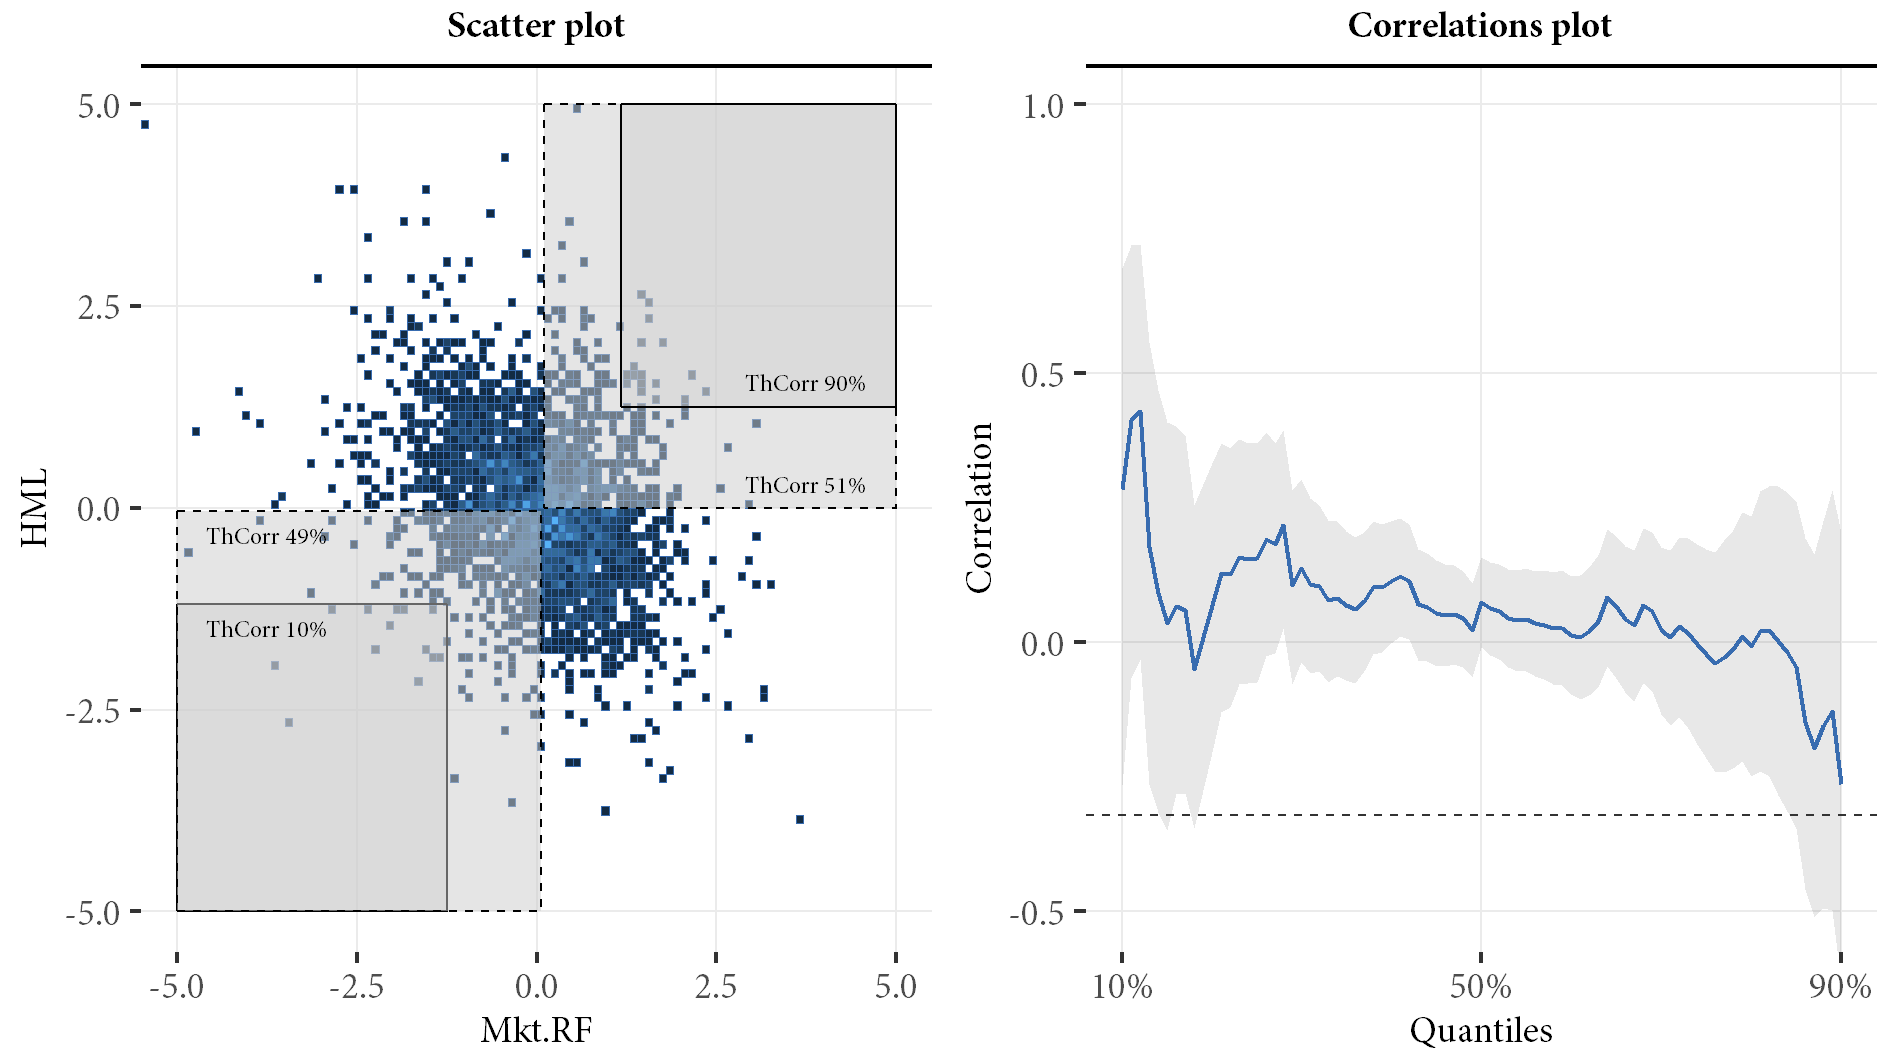
\includegraphics[scale=1]{graphics/threshold_explain_res.png}
  
\end{figure}

We now plot threshold correlations without the adjacent scatter graph. \autoref{fig:threshold1} displays threshold correlations for HML, CMA and RMW against eachother as well as against the the other factors Mkt.RF, SMB and Mom. We note that for most asset pairs, the threshold correlation is significantly different from the unconditional correlation coefficient, given by the dashed line.

We also note that there is asymmetry around the median for some factor pairs, including the Mom--CMA, RMW--HML, RMW--CMA, and to a lesser extent Mkt.RF--RMW asset pairs. For example, in the Mom-CMA asset pair, the threshold correlation jumps up for the first percentile below the median, indicating that the correlation is higher when both realize below the median than when both realize above the median. This type of asymmetric property, where downside (below the median) correlation is higher than upside correlation is unwanted, as it reflects a poorer diversification in bad times. The opposite type of asymmetry can be seen for the HML--RMW and CMA--RMW asset pairs -- when these factors simultaneously realize above the median, they are significantly more correlated. This, however, presents no diversification problem.

Although estimated with substantial uncertainty, the threshold correlation do not seem to be constant as $p$ approaches either zero or one. For example, the Mkt.RF--HML asset pair seems to have a downward pattern, where correlation is the most positive in the lowest percentiles of residuals and the most negative in the highest percentile of residuals. In fact, this pattern is unwanted from a diversification perspective, as series tend to coincide more in extreme negative events. 

As do the original return series, all residual factor pairs exhibit unconditional correlation of near or below zero, except for the CMA--HML pair which exhibits a correlation in excess of $0.60$. Additionally, the threshold correlation estimate is much closer to this unconditional correlation -- suggesting that the tails of this pair is similar to the average.

While the patterns in threshold correlations are interesting, we are careful not to draw conclusions regarding diversification benefit based on solitary threshold correlation graphs -- what is interesting is the total pattern, and our key point is that there seems to be tail dependence that should not be ignored in the copula specification.

\begin{figure}[H]
  \centering
  \footnotesize
  \caption{Threshold correlations of ARMA-GARCH standardized residuals, fitted on full dataset (1963--2016). 95\% confidence bounds taking the model as given. The unconditional correlation is given by the dashed line.}
  \label{fig:threshold1}
  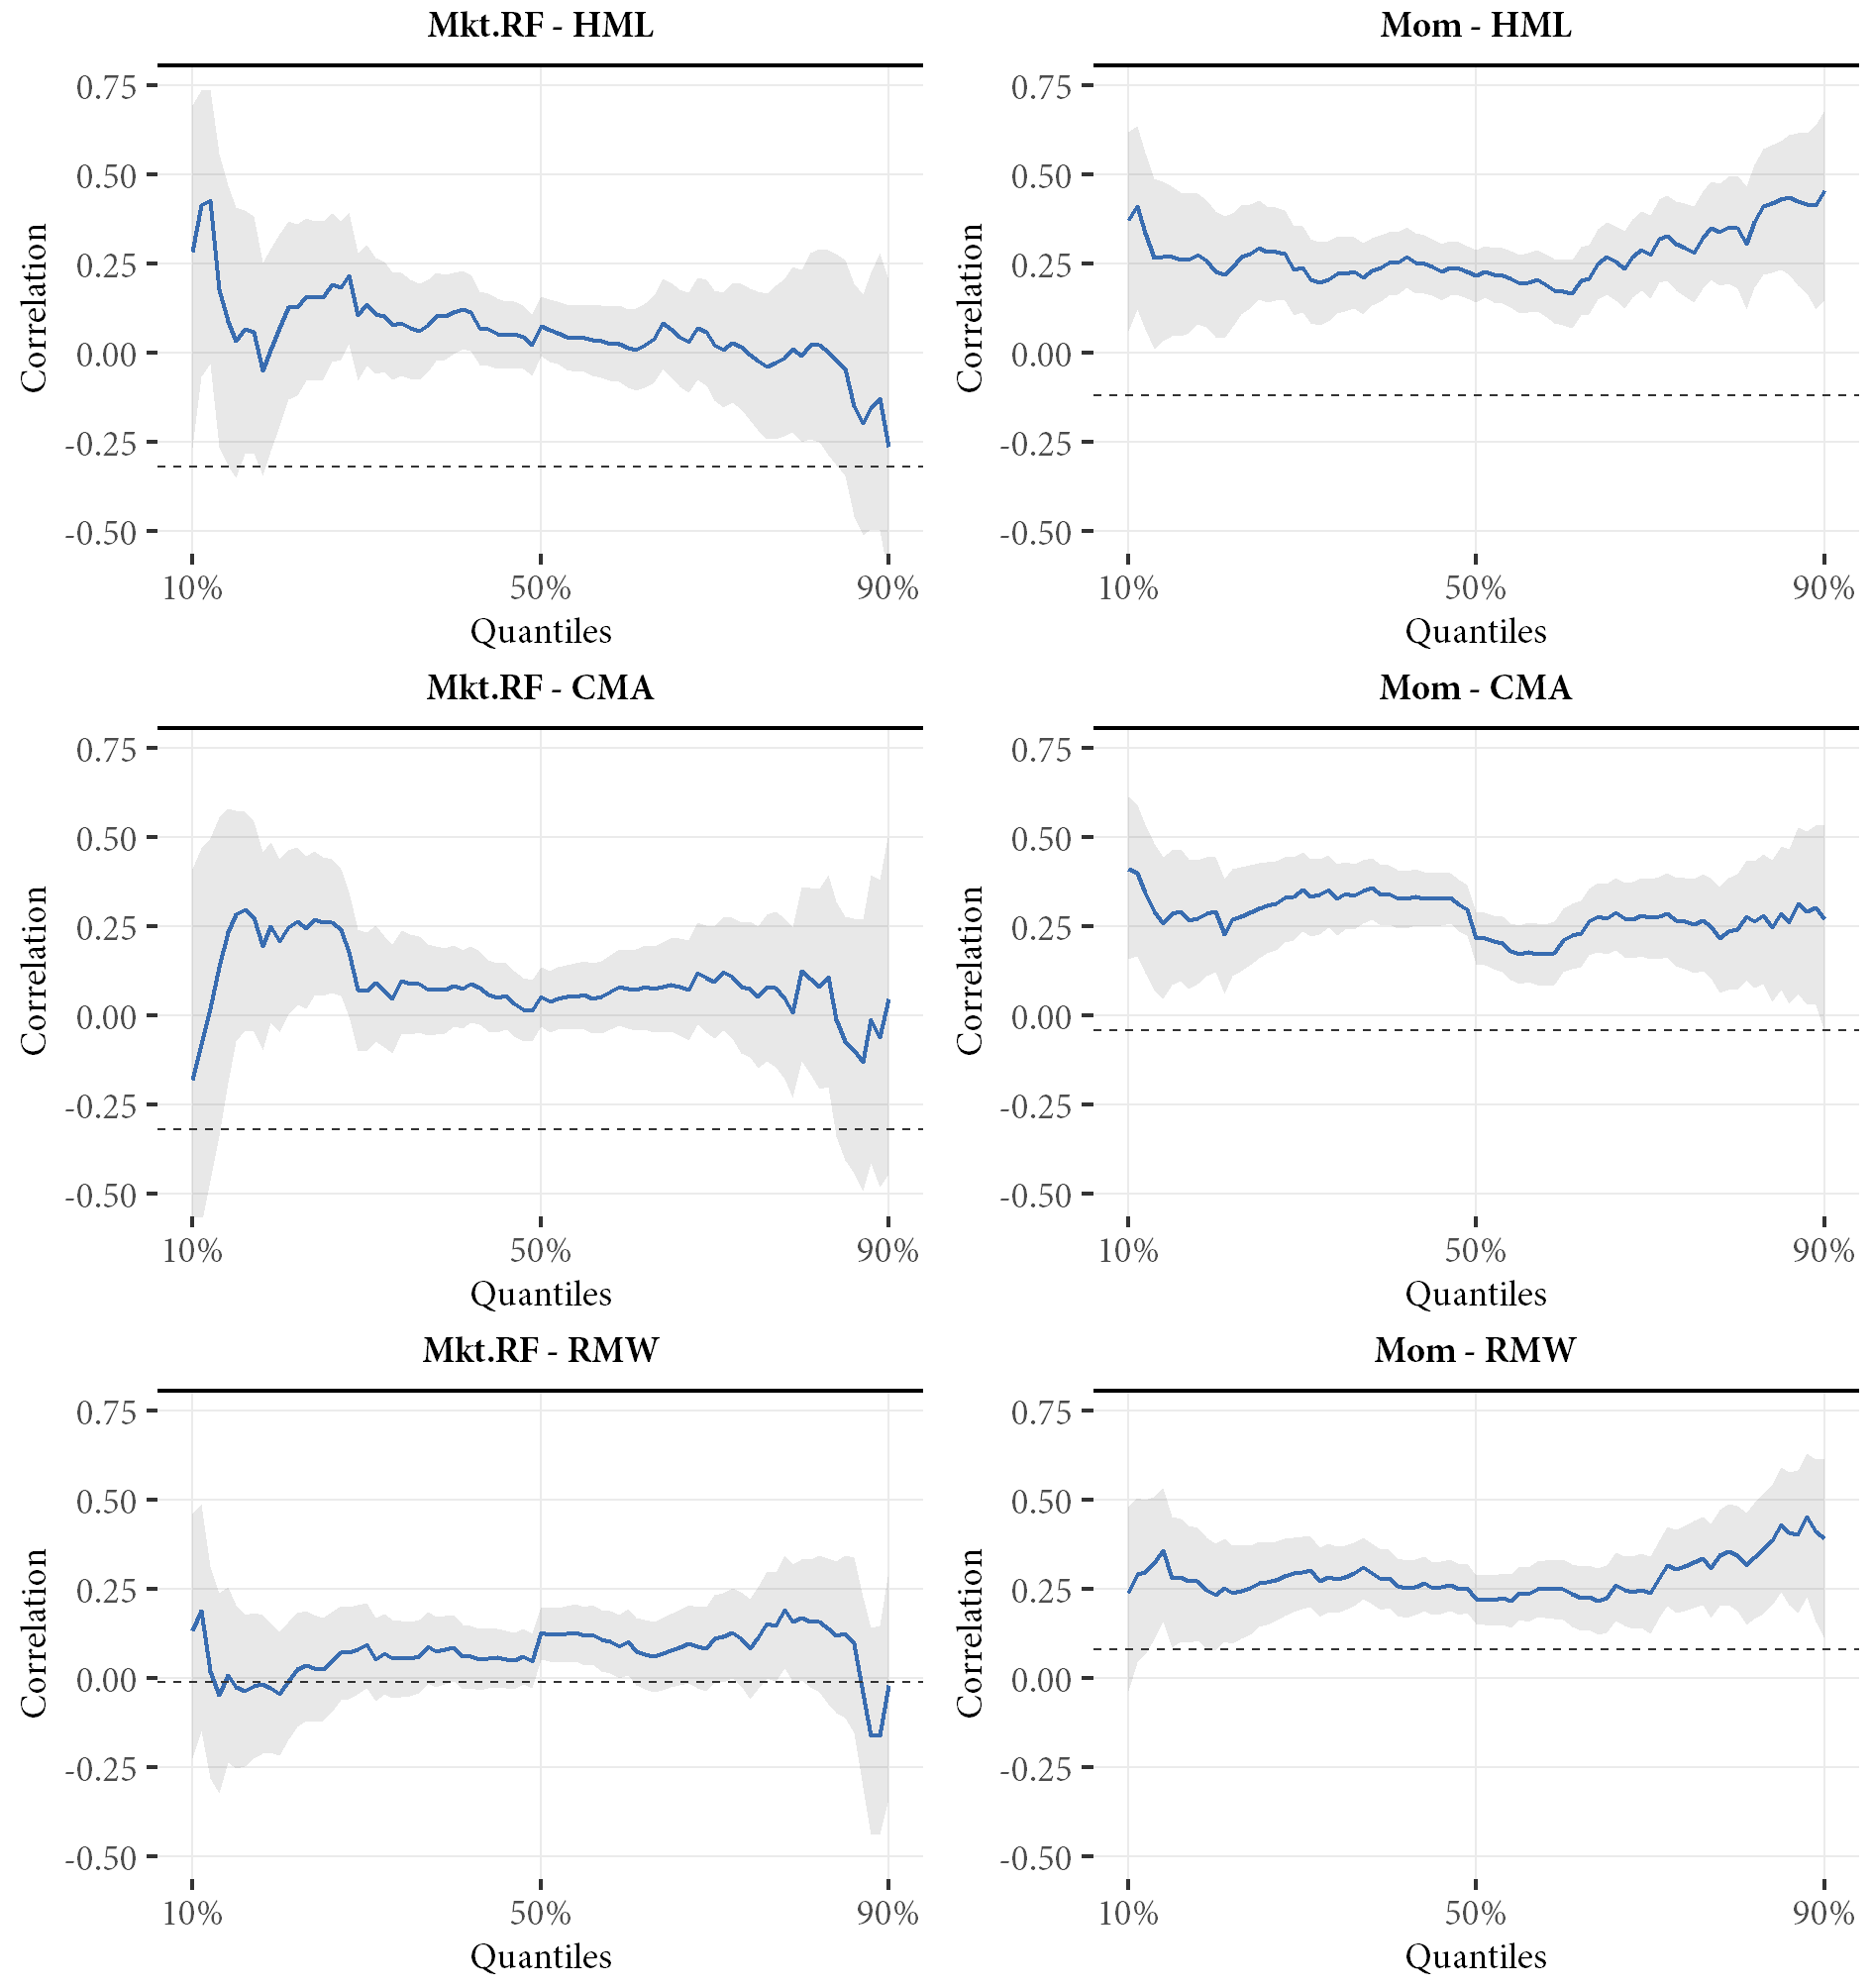
\includegraphics[scale=1]{graphics/threshold1.png}
\end{figure}

\begin{figure}[H]
  \ContinuedFloat
  \centering
  \caption{Threshold correlations of ARMA-GARCH standardized residuals (cont.)}
  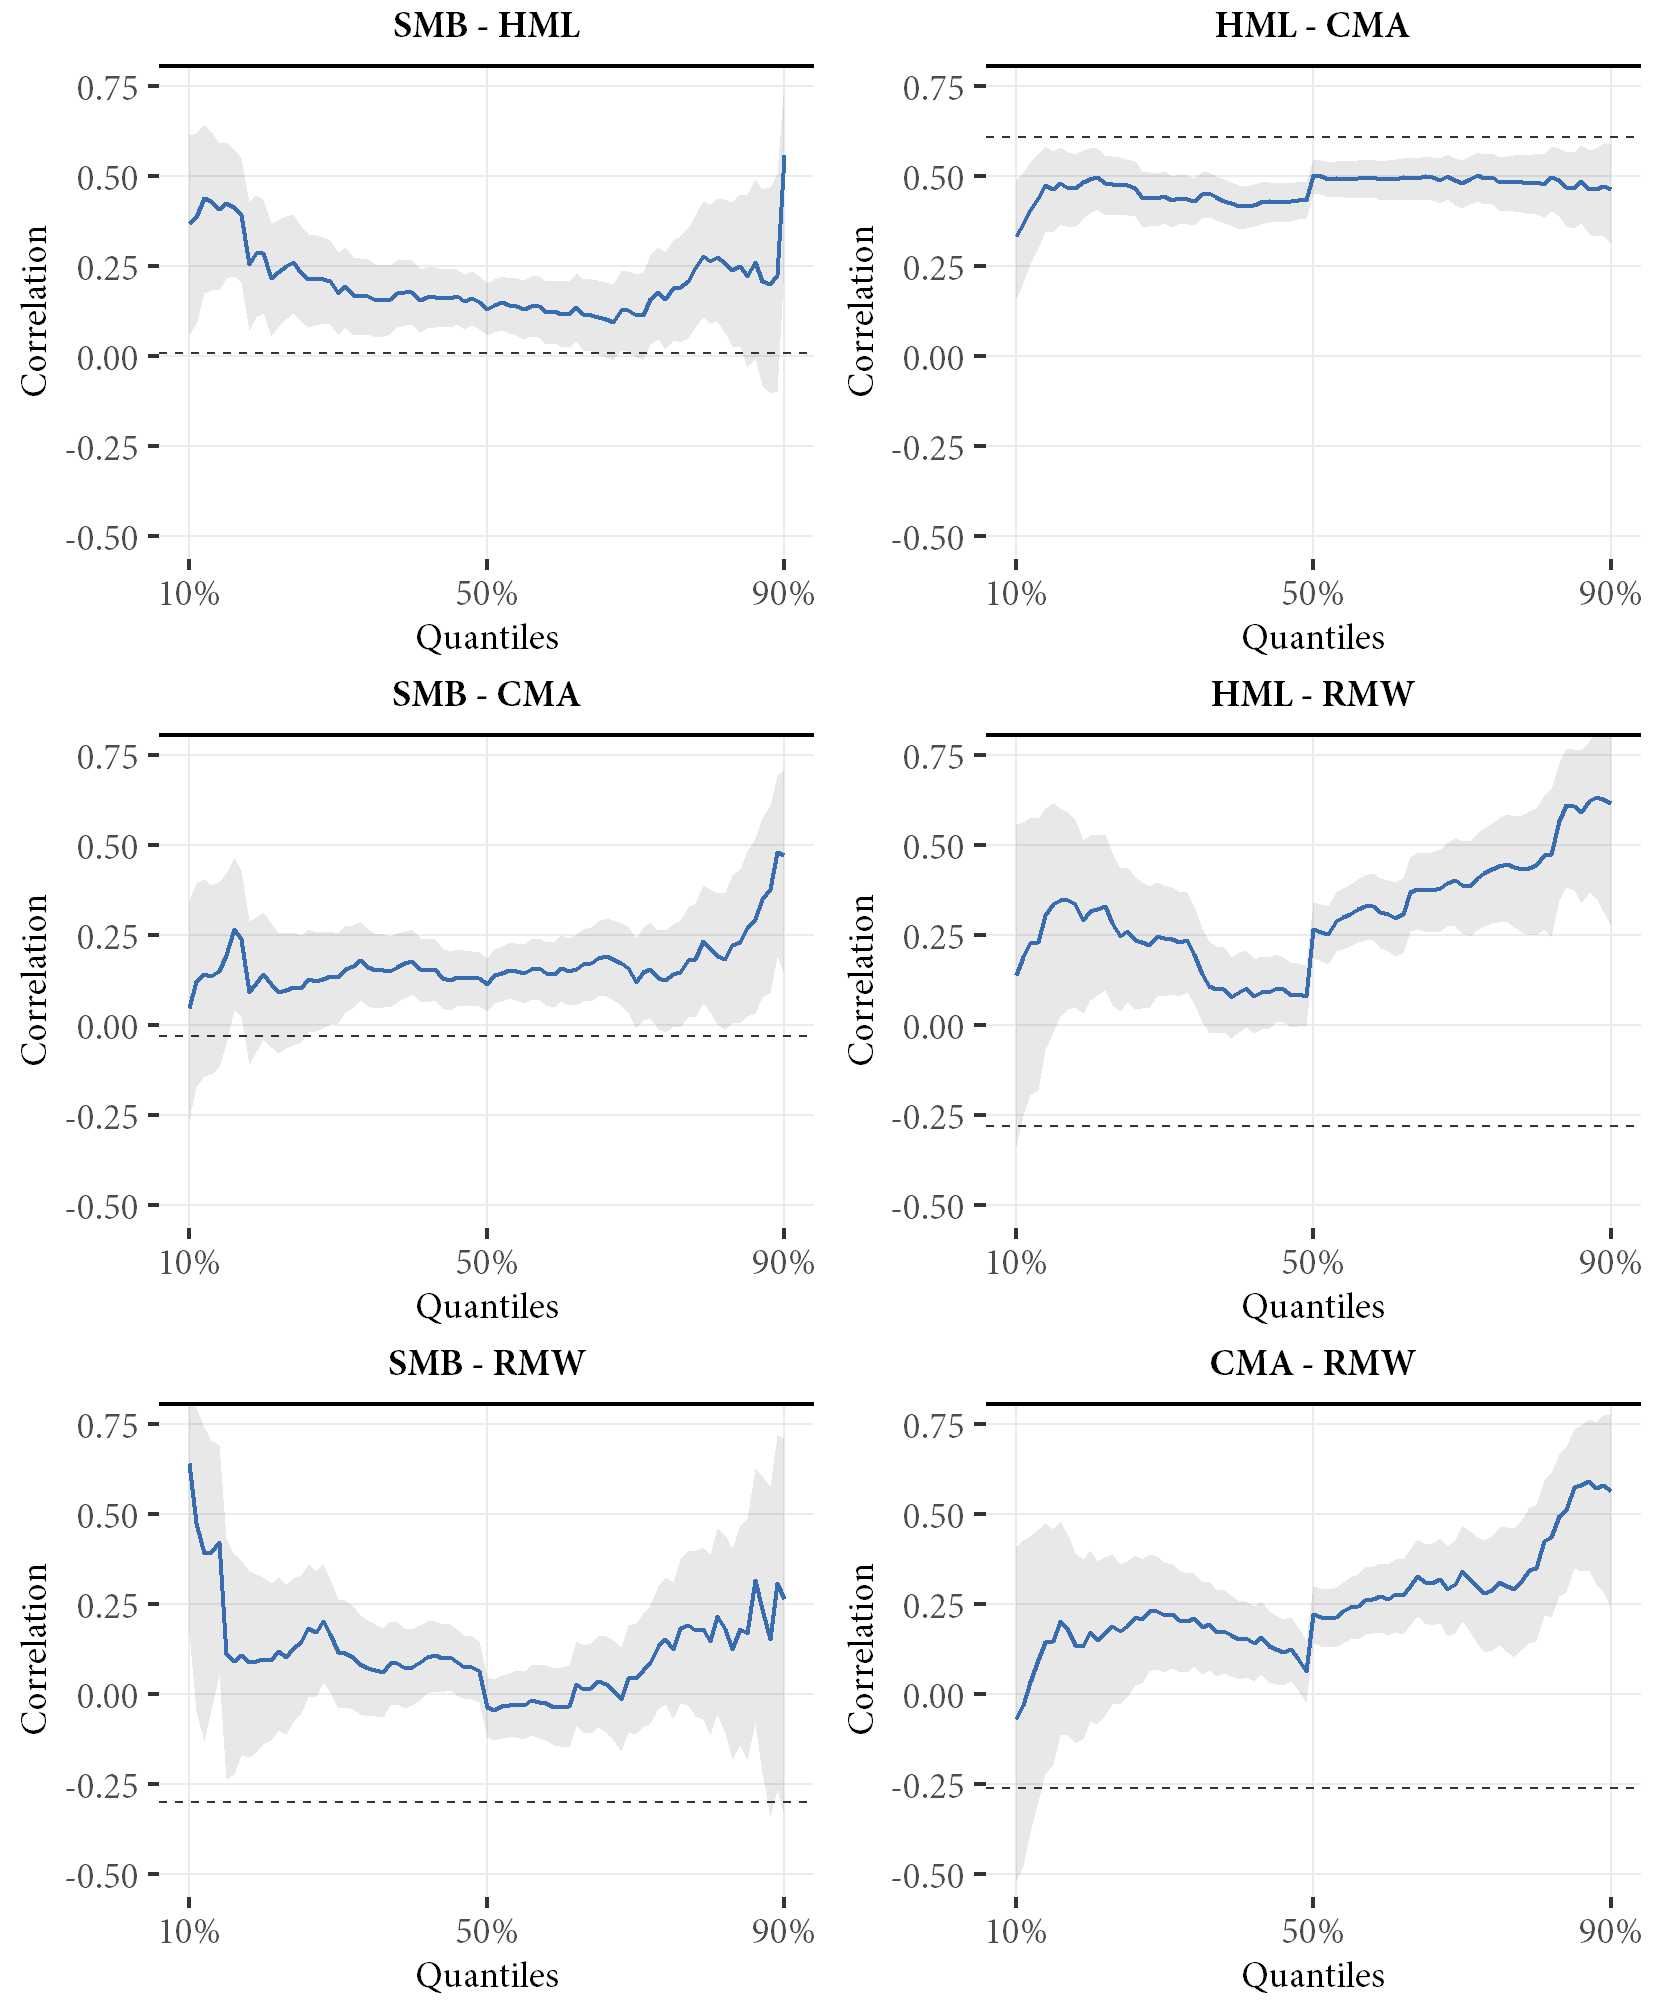
\includegraphics[scale=1]{graphics/threshold2.png}

  
\end{figure}

\subsubsection{Rolling correlations}

We compute rolling 52-week correlations between the factors on standardized residuals of our ARMA-GARCH models, according to the formula: 
\begin{align}
    RCorr(r_{i, t}, r_{j, t})_t^{52} = \frac{\sum^{t}_{t-51}(r_{i, t} - \bar{r}_i)(r_{j,t} - \bar{r}_j)}{\sqrt{\sum^{t}_{t-51} (r_{i,t} - \bar{r}_i)^2} \sqrt{\sum^{t}_{t-51} (r_{j,t} - \bar{r}_j)^2}}
\end{align}
where $r_i$, $r_j$ are the different pairs of the factor strategies' ARMA-GARCH residuals.\footnote{Rolling correlations for the returns themselves are available in the appendix.} Results are presented in ~\autoref{fig:rolling1}.
% plots
\begin{figure}[!ht]
  \centering
  \caption{Rolling correlations of ARMA-GARCH standardized residuals \\ \quad \\
   Rolling correlations are fitted on the full dataset (1963--2016). 95\% confidence bounds taking the model as given. The unconditional correlation is given by the dashed line.}
  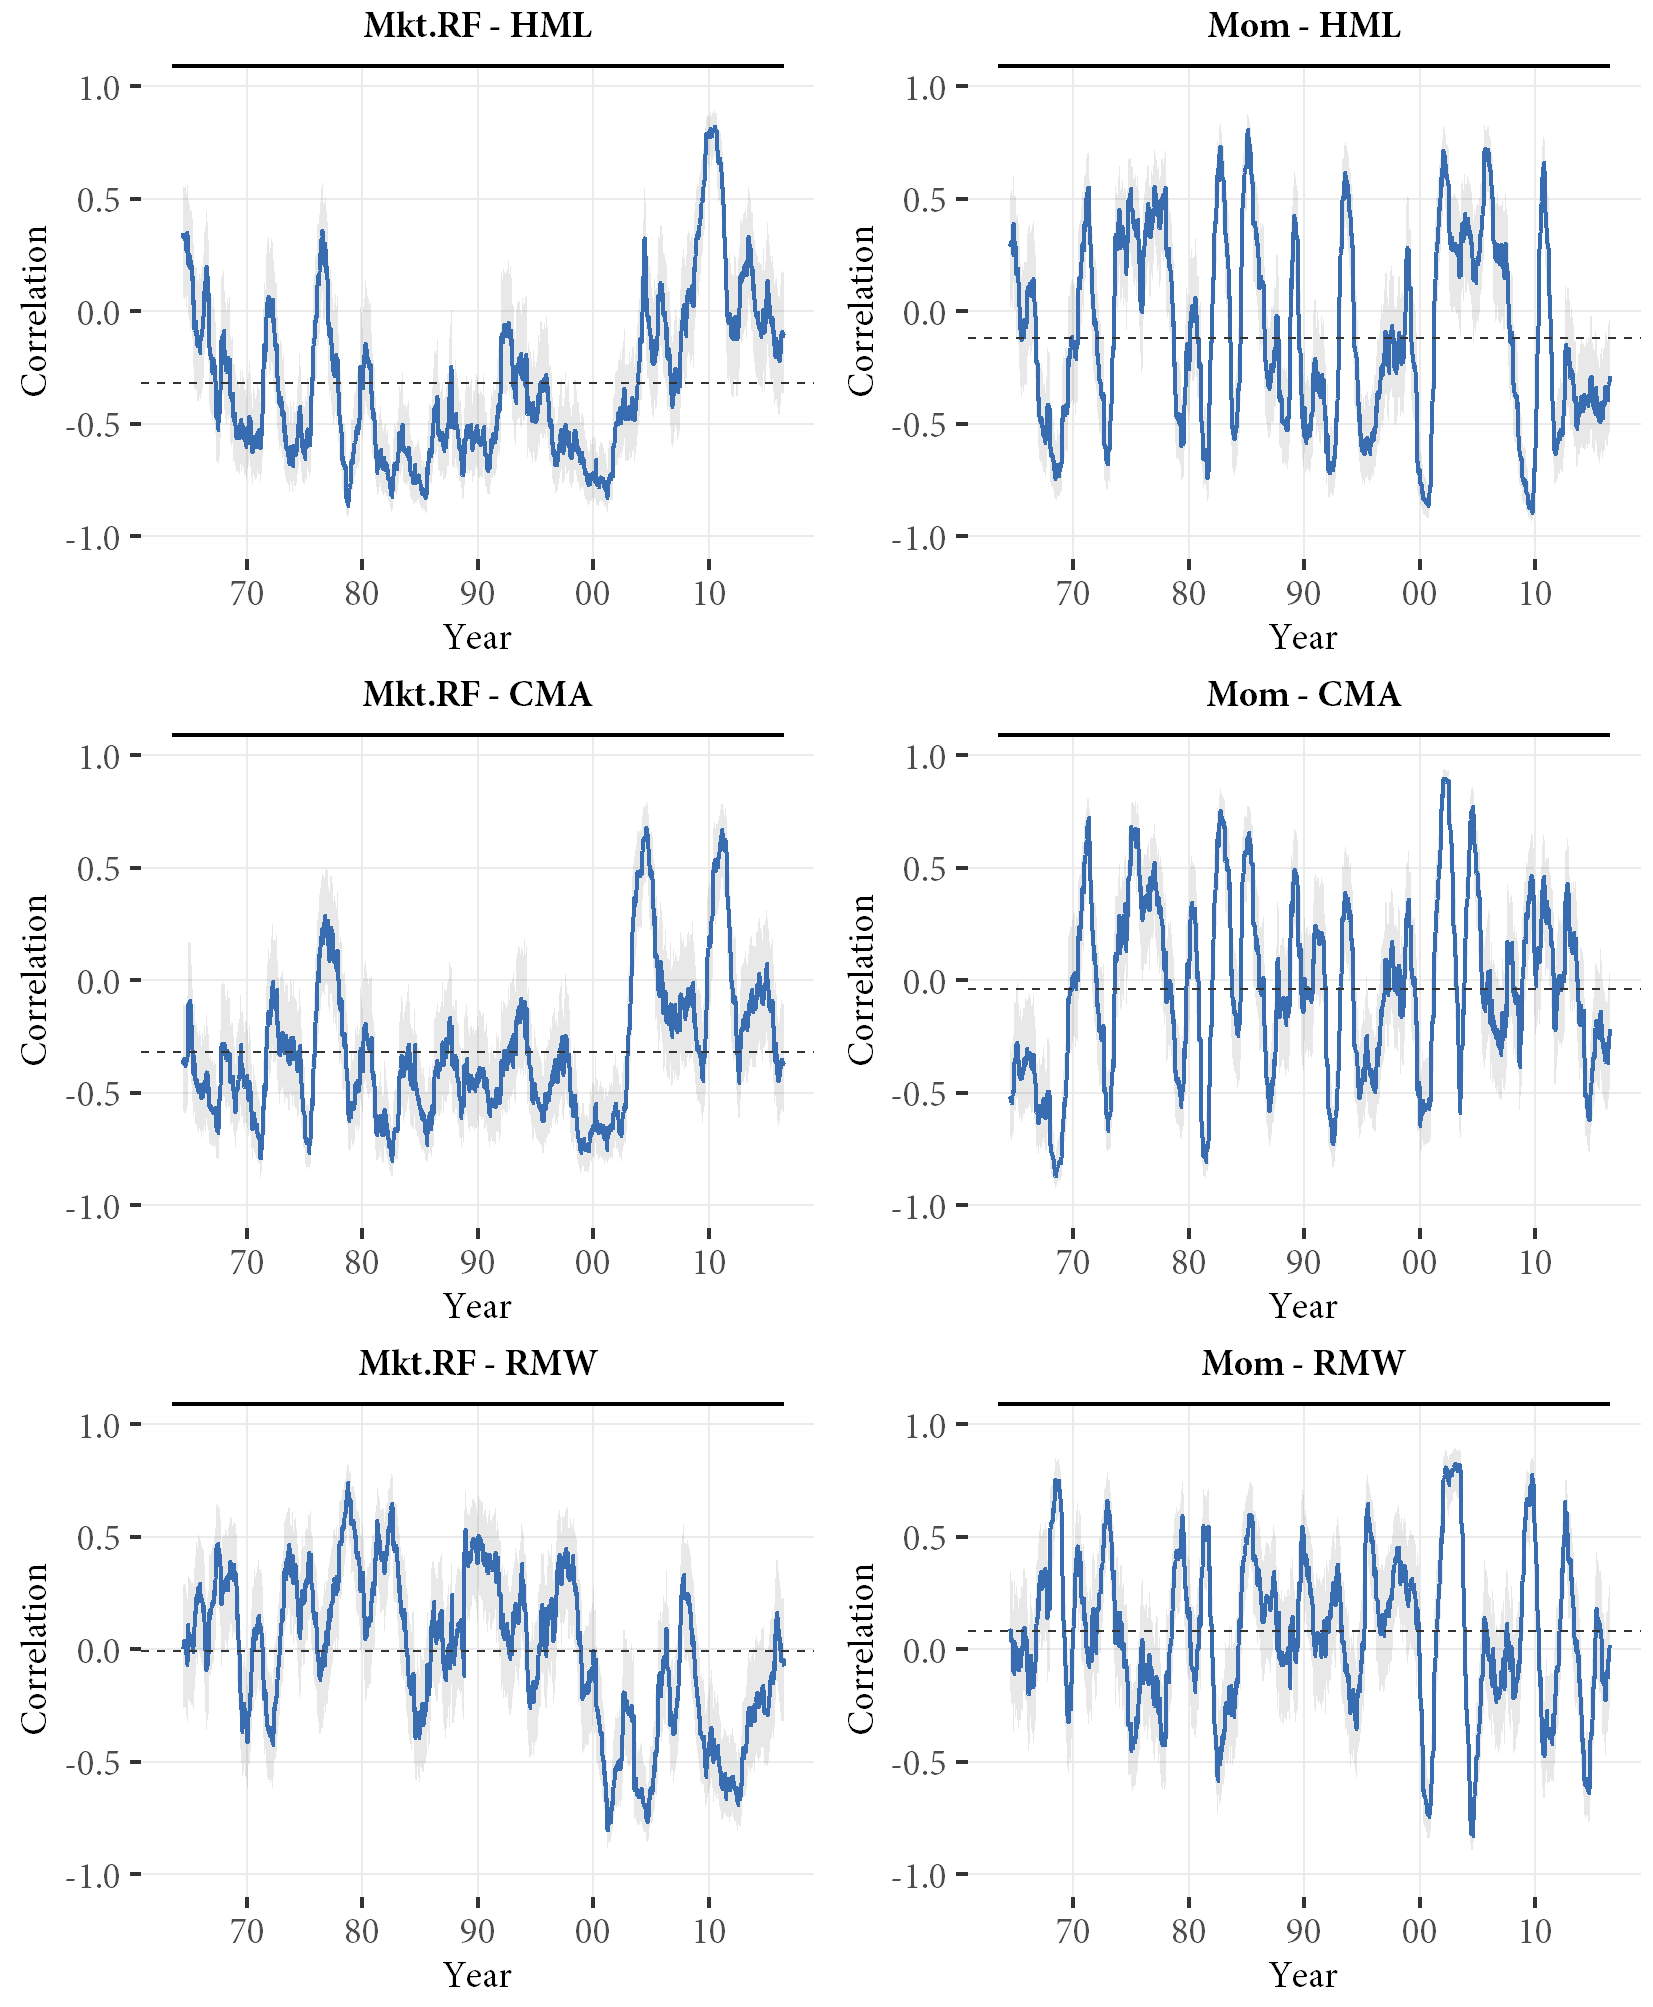
\includegraphics[scale=1]{graphics/rolling1.png}
  \label{fig:rolling1}
\end{figure}
\begin{figure}[!ht]
  \ContinuedFloat
  \centering
  \caption{Rolling correlations of ARMA-GARCH standardized residuals (cont.)}
  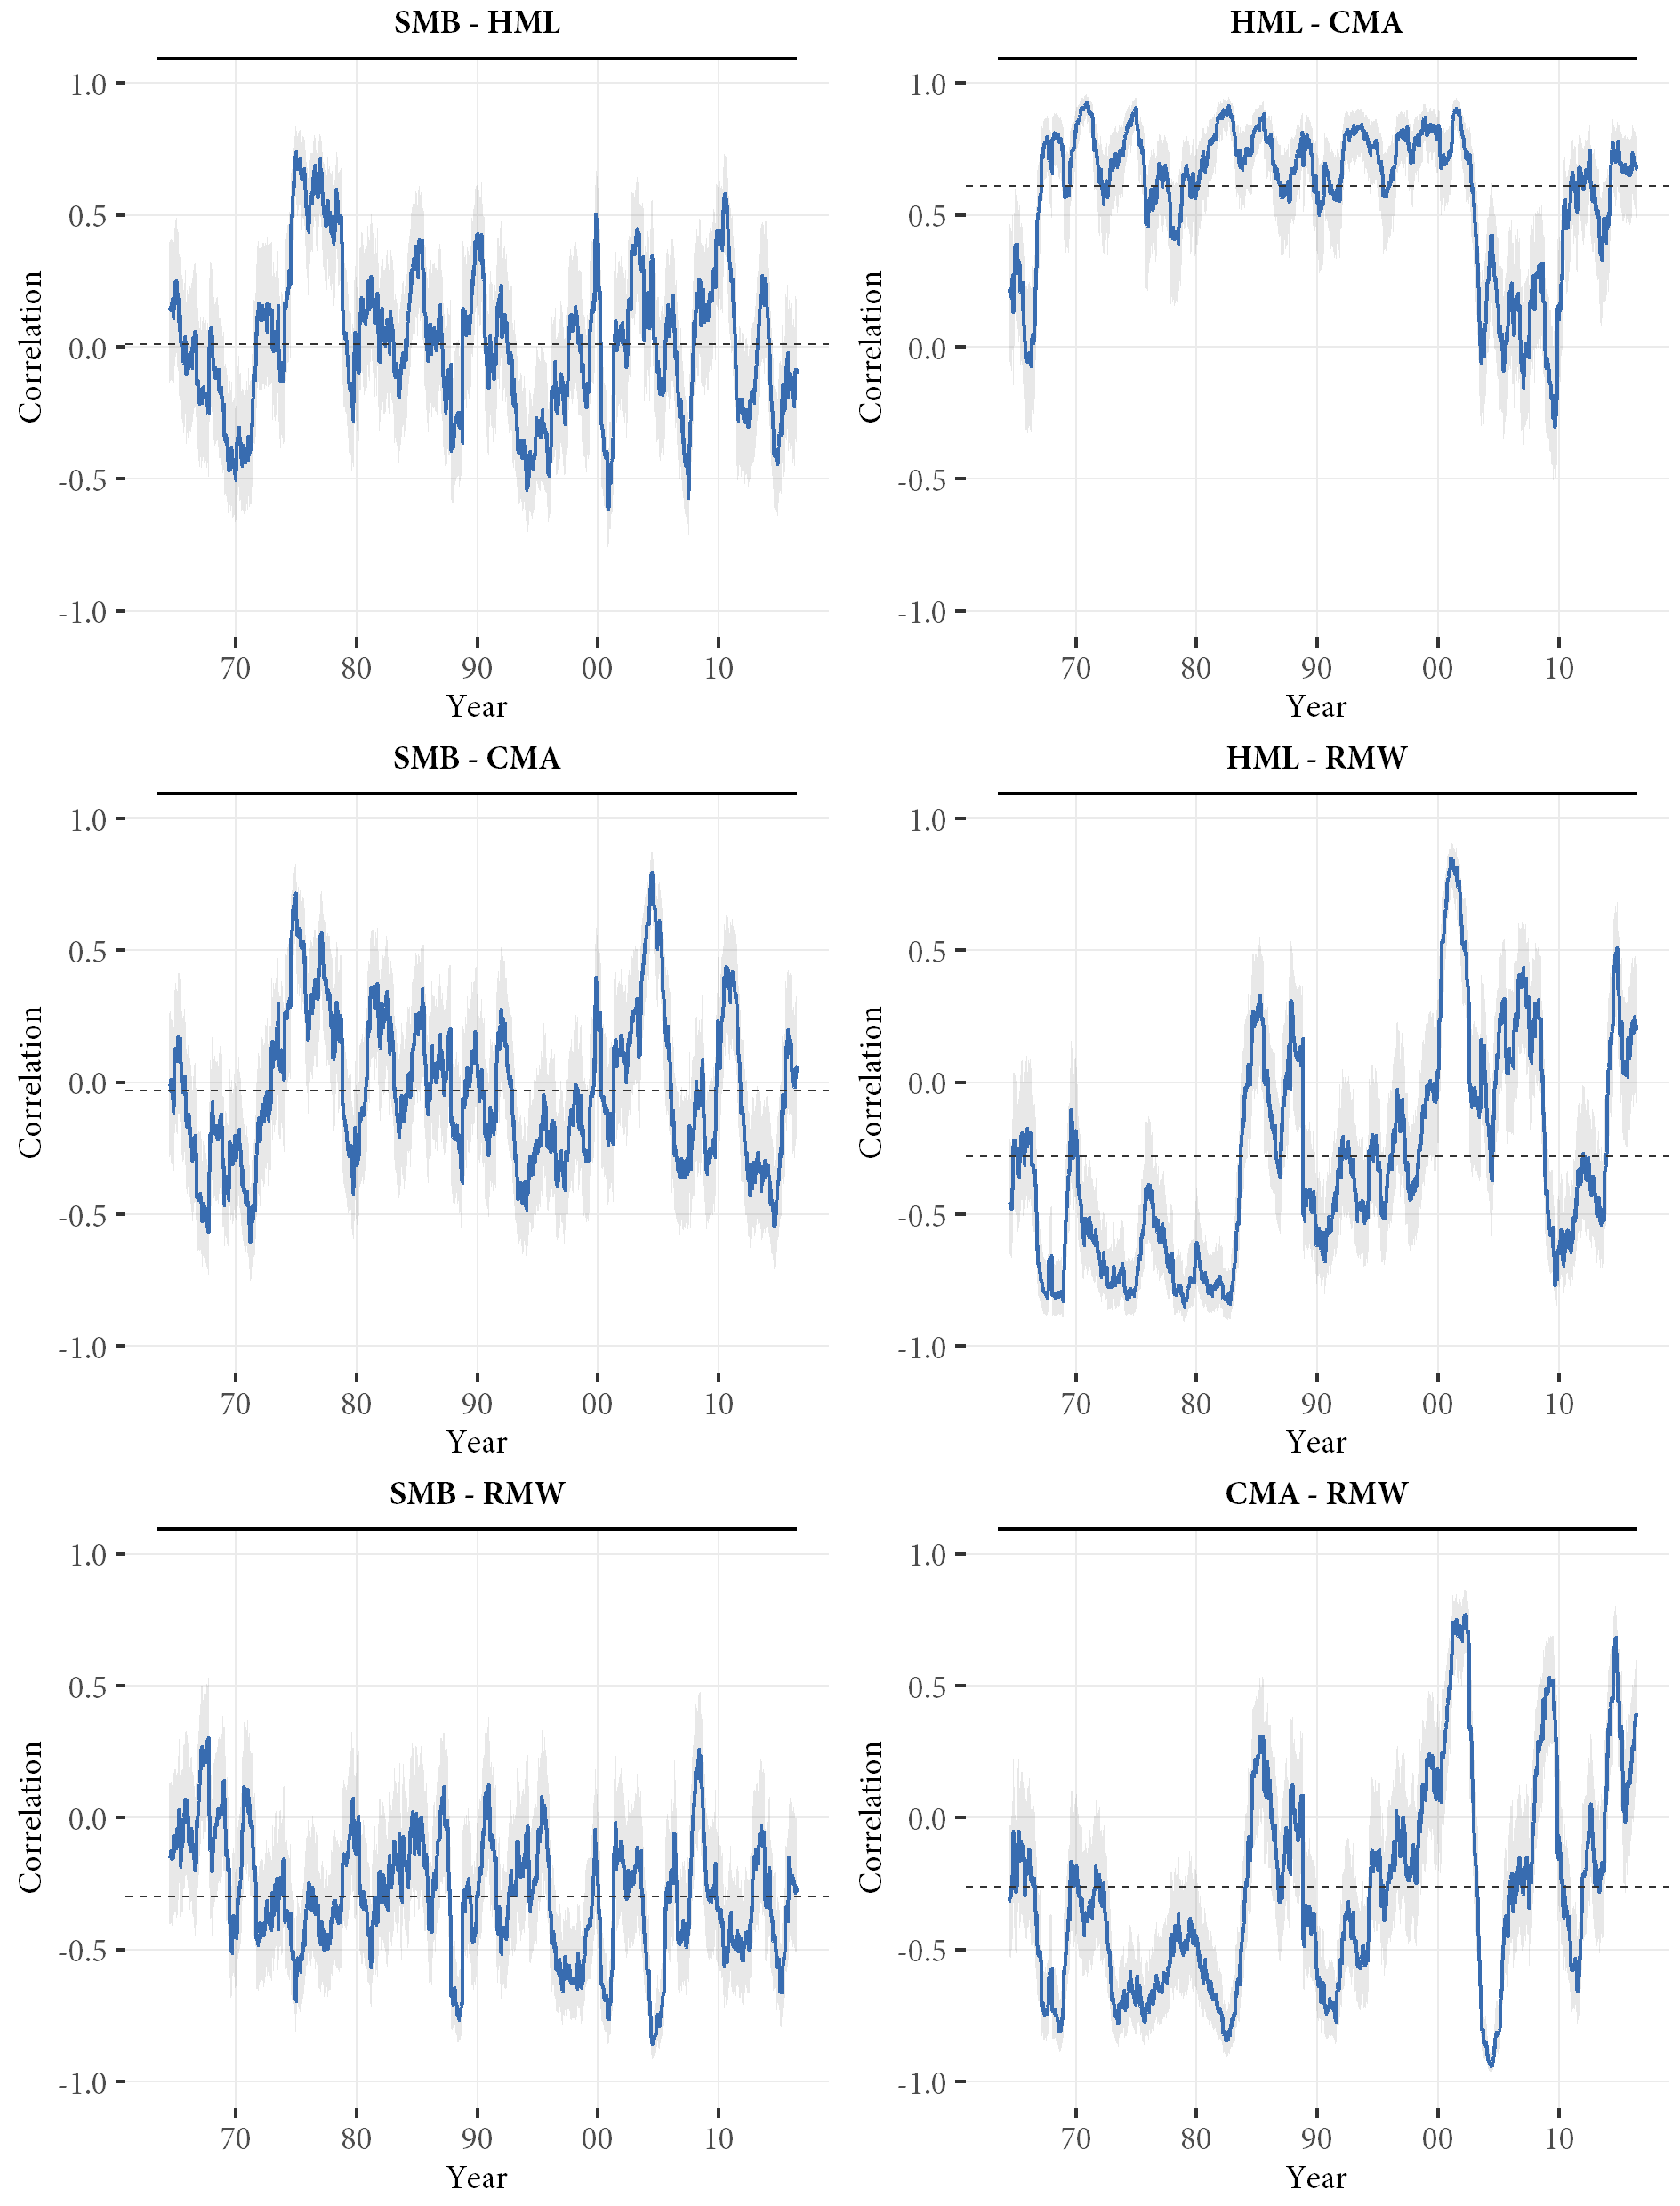
\includegraphics[scale=1]{graphics/rolling2.png}  
\end{figure}
% talk
First, we note that for most factor pairs, the rolling 52-week correlations are time-varying, and indeed appear to swing wildly. The unconditional correlation of Mkt--HML is negative in the studied time period, but rolling correlations range between -0.75 and 0.75. Also of note is the Momentum factor's rapid shifts between positive and negative correlations to the other factors. 

% Value and profitability in crisis times?
Second, by visual inspection, we see no obvious trend in the correlations between factor pairs, however, there are notable patterns around the 2000--2001 period -- the correlations of HML--RMW, CMA--RMW and Mkt--CMA appear to jump sharply. This is an indication that diversification benefits may be time-varying. Another interesting pattern is that the correlations of Mkt--RMW went down sharply around this period -- in line with the idea that profitable firms are stronger and better at weathering crises than the average firm~\autocite{NovyMarx2013}. The 2000--2001 period may represent a structural break in the dependency patterns between factors, with the appearance of persistent differences before and after -- however, there is not enough post-2000 data to support such a conclusion, yet.

Third, the HML and CMA factors again stand out as different to other factor pairs. The unconditional correlation is much closer to the rolling estimates than for other factor pairs, with a dip in the 2000--2010 period that appears to have gone away. Clearly, the HML--CMA pair is the most strongly correlated factor pair, even when considering specific time periods in the data.

Our key takeaway from the rolling correlations is that there seems to be persistency in the time-variation in correlations. This could be incorporated in the copula specification, which then needs to have a time-varying correlation matrix, $\Psi_t$.

% \subsubsection{Takeaways from Analysis of Multivariate Dependence}

% Univariate residuals appear to be white noise series with no remaining autocorrelation or volatility clustering. However, there is important dependence between residuals of different strategies. First, threshold correlations show that there is tail dependence -- in times when factor pairs simultaneously realize in their best and worst percentiles, correlations are significantly different from the unconditional correlations. In fact, threshold correlations are substantially higher than the unconditional correlations, which indicates that diversification benefits are smaller than expected when factors simultaneously experience bad (or good) times. Second, rolling correlations show that correlations between series are highly time-varying and seem to exhibit persistence. A copula model that incorporates both tail dependence and time-varying dependence is likely to improve on the description of joint returns.

% Both analyses also show that the HML-CMA asset pair is quite different from the other pairs, exhibiting a much higher and more stable dependence. Differently put, they look quite similar as opposed to any other factor pair, and the merit of including both in factor portfolios seems more unclear.

\label{sub:threshold_and_rolling_correlations_of_residuals}

% subsection threshold_and_rolling_correlations_of_residuals (end)
